%!TeX root= ../thesis.tex

\begin{abstract}
\ac{MJ} is a voting system where voters assign grades to candidates using an ordinal scale. The winner is the candidate with the highest majority-grade \textemdash which is the median of the grades received. This method has attracted increasing attention of french associations and political parties which have started to use \ac{MJ} for internal decisions or local elections. In particular LaPrimaire.org is a french association that uses \ac{MJ} to choose its candidate for the french presidential election. The vote is conducted in two rounds: in the first one the voters judge five candidates randomly picked; the five candidates with the highest medians pass at the second round as finalists and the voters are asked to judge them. Is the random selection of candidates a good elicitation technique? In this paper we explore the consequences of profile incompleteness and prove that this method can fail to elect the winning candidate of the complete profile. Furthermore, we perform experiments on randomly generated profiles and profiles following the grade distribution of a real voting scenario. We find that the probability of not selecting the winner of the full profile greatly decreases as the number of voters increases and we investigate how much of the grade vector we should know in order for this probability to be low. 
\end{abstract}

\section{Introduction}
\label{sec:intro}
\ac{MJ} is a voting method proposed by \citet{Balinski2007,Balinski2011} to elect one out of $m$ candidates based on the judgments of $n$ voters. The latter express their preferences by assigning to each candidate one of the following adjectives: Excellent, Very good, Good, Average, Mediocre, Inadequate, To be rejected. Those adjectives represent a common language whose semantic is assumed to be a shared knowledge among the voters carrying thus an absolute meaning. For each candidate the median of the grades she received is computed, this is called \textit{majority-grade}. The candidate with the highest majority-grade is elected. Ties are broken by considering the majority-grade of first order: one vote associated with the majority-grade of each tied candidates is removed and their medians are recomputed. The candidate with the highest new median is elected. If there is still a tie the process is repeated until a unique winner is found. 

In the last few years \ac{MJ} has being adopted by a progressively larger number of french political parties including: Le Parti Pirate, Génération(s), LaPrimaire.org, France Insoumise and La République en Marche.
%https://www.lopinion.fr/edition/politique/en-marche-teste-elections-jugement-majoritaire-mode-scrutin-tres-201884
"Mieux Voter" \citep{MV} is a french association that promotes the use of \ac{MJ} as voting method whenever a collective choice has to be selected: public administration, associations, companies. On their website it is possible to find all the citizens lists \textendash party lists that are not affiliated to any national political party \textemdash that used \ac{MJ} to rank their candidates during the local elections of 2020. In two cases, Bordeaux et Annecy, the candidate selected using \ac{MJ} was then elected as a mayor. 

In particular, LaPrimaire.org \citep{LaPrimaire} is a french political initiative whose goal is to select an independent candidate for the french presidential election using \ac{MJ} as voting rule. The association Democratech implemented the platform for the first time in 2016 in view of the 2017 presidential elections. The number of voters who participated in the election was $10676$ during the first round, and $32685$ during the second round. \commentOC{That’s pretty funny, it reads like everybody is cheating like hell, with this number of votes greater than the number of voters.}\commentBN{\href{https://twitter.com/meduza_en/status/1576937466652549121}{$https://twitter.com/meduza_en/status/1576937466652549121$}}

The procedure that they adopted consists of two rounds. In the first round each voter is asked to express her judgment, using \ac{MJ}, on five random candidates. At the end of this phase the five candidates with the highest medians are considered the finalists who qualify for the second round. In the second round each voter is asked to express her judgment, using \ac{MJ}, on all the five finalists. The candidate with the best median at the end of this phase is selected as representative for the presidential election.

In this paper we analyse this elicitation process of voters preferences. In particular, we investigate the consequences of randomness when asking the voters to judge candidates. We then search for more efficient techniques both in terms of communication cost \textemdash which can be quantified as number of questions per voter \textemdash and of fairness for candidates \textemdash which reflects the idea that a potential winner should not loose for lack of information.


\subsection{Related work}

One of the earliest uses of the median as an aggregator in voting theory can be identified in the \textit{middlemost} method proposed by \citet{Galton1907a,Galton1907b}. In particular, in situations where a group of people had to assess a damage, he suggested the median as the only method that does not suffer from over- or under-exaggerations.

We can consider the median grade as the highest level at which a candidate obtains the support of the majority of the voters. Starting for the highest grade $\delta$ we check if the majority of the voters assigned at least $\delta$ to some alternative. If this is not the case, we descend in the grading scale until such level $\delta^*$ is found. The grade $\delta^*$ is the median of grades associated to some alternative, and, since it is the first level we stopped at, it corresponds to the best possible median. This method was rediscovered several times and proposed under the name of Bucklin's rule \citep{Hoag1926}, Majoritarian Compromise \citep{Sertel1986,Sertel1999} and q-approval fallback bargaining \citep{Brams2001}. Moreover, when the number of grades is equal to two (approve, disapprove) then it is reduced to Approval Voting.

More recently \citet{Bassett1999} proposed the use of the median as voting rule for elections advocating for its robustness.
Several studies on the use of the median have been conducted. In particular, \citet{Bassett1994} and \citet{Gehrlein2003} study its manipulation. \citet{Barthelemy1981} survey mathematical problems and properties related to the notion of median in the context of cluster analysis and social choice theory. \cite{Nehring2022} analyze the median rule in judgment aggregation and they define a weighted median rule that is equivalent to \acs{MJ} except for the treatment of ties.

However, there is a significant concern that has never been analyzed when considering \ac{MJ}. Asking voters to provide a grade for each of the candidates can have a high cognitive and communicative cost. In situations where the set of alternatives is very large, voters may not be able to assign a significant and informed grades. \citet{Conitzer2005} studied the complexity of communication of some of the most common voting rules.
In these cases, elicitation strategies exist to retrieve the most relevant information. \citet{Konczak05} introduced the notion of possible and necessary winners. This paved the way for procedures that attempted to find necessary winners by asking voters the fewest questions possible \citep{Kalech2011}.
Considering scoring rules, \citet{Lu2011} suggested the use of minimax regret as a guide to the elicitation procedure. \citet{Bachrach2010} proposed a probabilistic approach. Several authors studied the complexity of determining when to stop the elicitation process for some of the most common voting rules \citep{Conitzer2002, Walsh2009}.
However, to the best of our knowledge, there are no works on preferences elicitation considering \ac{MJ}.

Very recently, \citet{Varloot2022} considered a version of \ac{MJ} under uncertainties in order to study its strategyproof properties. Their premise, however, is based on the fact that voters who are uncertain about the degree to assign to an alternative would instead assign to it a probability distribution. In other words, if a voter does not know whether to assign good or excellent to a certain alternative, then she may assign to it, for example, good with $\frac{1}{3}$ of the probability and excellent with $\frac{2}{3}$ of the probability. 
This approach requires the submission of even more information and is very far from our idea of incomplete knowledge.


\section{Notation}
\label{sec:complete}
Consider a finite set $N=\{i_1, \dots, i_n\}$ of voters (or judges) and a finite set $A=\{j_1, \dots, j_m\}$ of alternatives (or competitors). 
A \textit{common language} $\triangle = \{ \delta_1, \delta_2, \dots \}$ is a set of strictly ordered grades, and the notation $\delta_1 \geq \delta_2$ indicates that $\delta_1$ is a better or equivalent grade than $\delta_2$. A profile $P : A\times N \rightarrow \triangle$ is a $m$ by $n$ matrix of grades. Given any $N'\subseteq N$, the operator $\rho: \triangle^{N'} \rightarrow \triangle^{\card{N'}}$ defines an ordering function that given a vector of grades $P_j$ returns the vector ordered by decreasing grades.

Consider a set of alternatives $S\subseteq A$,
%where $|S|=s$ and $s \in \intvl{1,m}$ \textemdash the double brackets represent an interval in the integers. 
we denote by $P^S \in \triangle^{S \times N}$ a restriction of the profile $P$ to only the alternatives in $S$, $P^S \subseteq P$. Note that when $S=A$ then $P^S=P$.
%\commentOC{Could also write $\restr{P}{S × N}$, which leads to more generality, if restricting the users is also sometimes convenient.}

%We let $f: \triangle^{N} \rightarrow \triangle$ denote a function that assigns to any vector of grades a final grade. Given any $S\subseteq A$, a grading function $f^S: \triangle^{S \times N} \rightarrow \triangle^S$ returns a vector of final grades by applying $f$ to every alternative in $S$.
% the \emph{middlemost} aggregation function $f$, for each vector of grades $r_i= (r_1 , \dots, r_n )$ associated to the alternative $i \in \intvl{1,m}$, returns: 
%\begin{align}
%	f(r_i) &= r_{(n+1)/2} \text{ when n is odd,} \\
%	r_{n/2} \geq f(r_i) &\geq r_{(n+2)/2} \text{ otherwise.}
%\end{align}

We let $\fmaj:\triangle^{N} \rightarrow \triangle$, denote the \emph{majority-grade} function that associates to a vector of grades $\emptyset \neq v \in \triangle^{N'}, N' \subseteq N$ its median grade value: $\fmaj(v) = \rho(v)_{\floor{\frac{\card{v}}{2}} + 1}$. Note that in case $\card{v}$ is even, two medians could be used, but, as in \citet{Balinski2011} definition, the lower grade is picked. 

%Given any $S\subseteq A$, by applying $\fmaj$ to all vectors of grades associated to the alternatives in $S$ we obtain the corresponding grading function $\fmaj[S]$. Formally, $\fmaj[S](P^S)_j = \fmaj[S](P^S_j)$. The $j$-\emph{th} element of the resulting vector is the median of the ordered vector of grades associated to the $j$-\emph{th} alternative. 
%%Because $f^S_{maj}(P^S)_i$ depends only on $P^S_i$ we write $f^S_{maj}(P^S_i)$. \commentOC{I am not sure I follow. You already have a notation for this, namely, $\fmaj(P^S_i)$, isn’t it?}
%Moreover, when we consider the complete profile (when $S=A$) we will write $\fmaj(P_j)$ instead of $\fmaj[A](P^A_j)$.
%\commentOC{I doubt that the general $f$ is actually useful, you only seem to use $f$ maj.}
%\commentOC{The argument doesn’t seem correct to me, in $\fmaj[A](P^A_j)$.}
%\commentOC{I find it confusing to use the same symbol ($\fmaj$) for two quite related but distinct functions.}
%i.e. it corresponds to the lower middlemost.

Given any $S\subseteq A$, the winner function $\Fmaj[S]:\triangle^{S \times N} \rightarrow A$ %$F^S_{maj}:\triangle^{S \times N} \rightarrow 2^A \setminus \emptyset$
is a function that given $|S|$ alternatives and their median grade, selects the alternative with the highest median grade as winner. We can define it as  $\Fmaj[S](P^S) = \argmax_{j\in S}\fmaj(P^S_j)$ assuming it is a singleton. 
For brevity, we will write $\Fmaj$ when considering $S=A$.
To avoid adding further complexity to the notation, we describe only informally what happens in case multiple alternatives are tied for the highest median grade $h$, thus, when $\argmax_{j\in S}\fmaj(P^S_j)$ is not a singleton.
In this case, ties are broken by removing one $h$ grade from the vectors of grades of each tied alternative, recomputing the new median grade and repeating the process until one unique winner is found or there are no more grades to remove. When $n$ is odd, this is equivalent to take the next element after the median, i.e. the one at index $(\floor{\frac{n}{2}} + 1) +1$. If there is still a tie we then look at the previous element before the median, i.e. the one at index $(\floor{\frac{n}{2}} + 1) -1$, and keep alternating until the tie is broken or there are no more elements in the vector. When $n$ is even the element before the median, i.e. the one at index $\floor{\frac{n}{2}}$, is taken first and, if there is still a tie, then the element after the median is considered, i.e. the one at index $\floor{\frac{n}{2}} + 2$, and so on. If after applying the mechanism there are still ties we break them using an arbitrary ordering defined on all alternatives, e.g. lexicographical order.

Similarly to the winner function, given any $x \in \intvl{1,m}$, we can define a more general \emph{selection function} $F^S_x:\triangle^{S\times N} \rightarrow \powersetz{A}$, where $\powersetz{A}$ is the powerset of $A$ excluding the empty set, that selects exactly the $x$ alternatives with the $x$ highest median grades. Thus, $F^S_x(P^S) = \Fmaj[S](P^S) \cup \Fmaj[S'](P^{S'}) \cup \dots \cup \Fmaj[S^{k-1}](P^{S^{k-1}})$ where $S'= S \setminus \Fmaj[S](P^{S})$, $S''= S \setminus \Fmaj[S](P^S) \setminus \Fmaj[S'](P^{S'})$ etc.


\subsection{Incomplete knowledge}
In order to analyze the elicitation procedure used by LaPrimaire.org, we need to adapt the notation just described to incomplete profiles. 
Let $\Pbar$ be our knowledge about the profile $P$.
The voters have full knowledge of their own judgments but we ignore them; our goal is to elicit them by questioning the voters starting from zero knowledge.
We introduce an additional grade $\dbar$, and, given a language $\Delta$, $\dbar< \delta, \forall \delta \in \Delta$.
%\commentBN{I think we should avoid to say this but rather add in $\bar{F}$ that the $\dbar$ are excluded.}
The common language in the incomplete knowledge setting is then $\overline{\triangle}=\triangle \cup \dbar$. Voters cannot use this grade to express their judgment over an alternative and it does not count in the computation of the median grade as we will explain formally. We refer to the grades in $\triangle$, the ones used by voters, as "defined" grades.

The starting knowledge is represented by a matrix $m\times n$ of $\dbar$ grades. Given $k \in \N$, we define with $K_i \subseteq A$ a set of $k$ alternatives that we ask the voter $i\in N$ to evaluate. 
After having asked every voter in $N$ to judge $k$ candidates, we obtain an \emph{incomplete profile} $\Pbar\in \overline{\triangle}^{A \times N}$, that is a matrix $m \times n$ of grades of which $kn$ are "defined".
Note that when $k=m$, the resulting profile $\Pbar$ corresponds to the complete profile $P$. Let $C(\Pbar)$ be the set of all completions of $\Pbar$ obtained by substituting all $\dbar$ grades with "defined" ones, note that $P \in C(\Pbar)$.
%if we want to define $C(\Pbar) = \{P' \in \triangle^{m \times n} \suchthat \restr{\Pbar}{\triangle} \subseteq P'\}$ then we introduce $\restr{\Pbar}{\triangle} = \Pbar \cap (A \times N \times \triangle)$
 
%If $K_i=K_l, \forall i,l\in N$, i.e. if we ask all voters to judge the same $k$ alternatives, then we have complete knowledge restricted to this set of candidates. We denote with $P^{K_i}$ the restriction of the complete profile $P$ to only the alternatives in $K_i$.
%\commentOC{I wonder if this notation will be useful.}

Let $g:\overline{\triangle}^N\rightarrow \bigcup_{N' \subseteq N}\triangle^{N'}$ be a \commentOC{the} function that given an incomplete vector of grades $q \in \overline{\triangle}^N$, thus $q \subseteq N × \bar{\triangle}$, returns the vector composed only of the "defined" grades. 
%$g(q) = \restr{q}{N × \triangle}$ \commentOC{This should be $q \cap (N × \triangle)$, but anyway as above this may be more complexity that what we do with this afterwards justifies, so perhaps omitting what $g$ is formally (especially considering that this union is not straightforward to understand) may be beneficial to the reader.}.

%The operator $\overline{\rho}$ defines a restricting ordering function that given $\overline{P_i}$, an incomplete vector of $n$ grades, returns the correspondent complete vector restricted to its $x$ "defined" grades decreasingly ordered: $\overline{\rho}(\overline{P_i})=\rho(d(\overline{P_i}))$. \commentBN{Not sure this is necessary.}

The \emph{majority-grade} for incomplete profile $\fmajbar: \overline{\triangle}^N \rightarrow \triangle$ corresponds to $\fmaj$ that only considers the "defined" grades in the computation of the median. Indeed, consider an incomplete grade vector $\overline{P}_j$ and let $P'_j=g(\Pbar_j)$ be the partial vector of $\overline{P}_j$ of only "defined" grades, then $\fmaj(P'_j) = \rho(P'_j)_{\floor{\frac{\card{P'_j}}{2}} + 1}$.
\commentOC{I suppose you mean to apply $\rho$ on $P'_j$. Also, your definition makes sense more generally for any $P'_j$ of the right type, not just when $P'_j = g(…)$. In fact, this $f$ is already defined!}
\commentOC{The domain of $\fmajbar$ should be the incomplete profiles; $P'$ is not defined; and $j$ does not seem relevant here. Anyway, same suggestion as above: omit the formal definitions.}\commentBN{I think it's correct now.}
\commentOC{Aren’t you willing to define $\fmajbar$ here? You’re actually defining $\fmaj$. Also, the argument of $\fmajbar$ should be an incomplete vector. And, it is not said what happens if $P'_j = \emptyset$, i.e., when the argument contains only undefined grades.}
In a similar fashion, we can define $\Fmajbar[S](\Pbar)=\argmax_{j\in S}\fmajbar(\Pbar^S_j)$ and, given a value $x\in \intvl{1,m}$, the selection function of the $x$ best alternatives is $\overline{F}^S_x(\Pbar^S) = \Fmajbar[S](\Pbar^S) \cup \Fmajbar[S'](\Pbar^{S'}) \cup \dots \cup \Fmajbar[S^{x-1}](\Pbar^{S^{x-1}})$ where $S'= S \setminus \Fmajbar[S](\Pbar^{S})$, $S''= S \setminus \Fmajbar[S](\Pbar^S) \setminus \Fmajbar[S'](\Pbar^{S'})$ etc.

To summarize the elicitation process we want to investigate, starting with zero knowledge, each voter is asked to evaluate $k$ candidates. Given the partial information at our disposal, we are able to define the "known" median grade for each alternative by applying $\fmajbar(\Pbar_{j}), \forall j\in A$. We can then use the \emph{selection function} $\overline{F}_k$ to select the $k$ alternatives with the highest "known" median grades. We denote this set of alternatives with $K=\overline{F}_k\subseteq A$. The alternatives in $K$ will be presented to all voters, who must provide a grade for each of them, thus obtaining a restriction of the complete profile to this subset of $k$ alternatives. From here, we can use $\Fmaj[K](P^K)$ to select the winning alternative of the restricted profile $P^K$.

%I'm not sure the following is relevant
%
%Given the set $\tilde{K}=F^S_k(g(\Pbar^S_j))$ of the best $k$ alternatives, every voter is then asked to judge all the candidates in $\tilde{K}$. 
%\commentOC{$i$ is not defined; and there may be a type incompatibility between the result of $g$ and the domain of $F^S_k$.}
%
%This process results in a restriction $P^{\tilde{K}}$ of the complete profile $P$. It is important to mention that when we ask the voters to judge an alternative $i\in \tilde{K}$ we assume that they report their preference as they would have stated it when asked about $P$. In other words, $P^{\tilde{K}}_{i} = P_j$ for any $i \in \tilde{K}$.
%\commentOC{The formal part of this does not look like your informal hypothesis.}
%
%Please note that $P^{\tilde{K}}$ is a complete matrix of $kn$ grades and that we fall back to the complete profile case, thus, we apply the \emph{majority-grade}, $\fmaj[\tilde{K}]$, function to $P^{\tilde{K}}$ to determine the median grades and then the winner function $\Fmaj[\tilde{K}]$ to select the winner. 
%For simplicity we denote by $\overline{W}_{\overline{P^k}} \subseteq A$ the results of this process.

\begin{remark}
	Because we are interested into investigating \acs{MJ}, we are going to use an alphabet with the same size of the one proposed by \citet{Balinski2011} which is composed of the following adjectives: To be Rejected, Inadequate, Mediocre, Average, Good, Very Good, Excellent. For brevity we are gonna rename those adjectives respectively from $\delta_1$, corresponding to To be Rejected, to $\delta_7$, corresponding to Excellent. Therefore, $\triangle=\{\delta_1,\delta_2, \delta_3,\delta_4,\delta_5,\delta_6,\delta_7\}$ 
\end{remark}

\section{Reasoning on incompleteness}
Let us now consider the effects of incomplete knowledge on the selection of a winner. In particular, we want to prove that if we consider an incomplete profile and take the $k$ alternatives with the highest median grade, with any $k$ being between $1$ and $m-1$, it is possible to miss the winner of one of its completion. 
This is important because in the elicitation process implemented by LaPrimaire.org, only the full grade vectors of the $k$ alternatives with the highest median grade are considered. Clearly, if the winning alternative in the complete profile is in this set $K \subset A$, then she will also be the winner of the incomplete profile. This is because the voters will be asked to provide a grade for all those $k$ alternatives, providing thus a restriction of the complete profile to only the alternatives in $K$, i.e. $P^K$. If a candidate is a winner for a complete profile, then she is also a winner for any of its restrictions that include her.
Note that this is not true in case of multiple winners where ties that cannot be broken by tie-breaking procedures and for which arbitrary ordering is, therefore, necessary. In what follows we assume the absence of such ties.
We want to show that it is possible for the winning alternative of the complete profile not to be included in this subset $K$ of alternatives.

	\begin{theorem}
		\label{th:notinK}
		Given a set $A$ of alternatives $m\geq 2$, a set of voters $N$ and a value $k\in \intvl{1,m-1}$, there exist a complete profile $P$ and an incomplete profile $\Pbar$ such that $P \in C(\Pbar)$ and $\Fmaj(P) \nsubseteq \overline{F}_k(\Pbar)$.
	\end{theorem}
	\begin{proof}
		Consider the following complete profile $P$
		\begin{center}
			$
			\begin{array}{ccccc}
				& i_1 & i_2 & \dots & i_n \\
				j_1 &	\delta_7 & \delta_7 & \dots & \delta_7 \\
				j_2 &	\delta_6 & \delta_6 & \dots & \delta_6 \\
				. &	\delta_6 & \delta_6 & \dots & \delta_6 \\
				j_m &	\delta_6 & \delta_6 & \dots & \delta_6 \\
			\end{array} \quad,
			$
		\end{center}
		where all voters judge all alternatives $\delta_6$ except for the alternative $j_1$ which is judged $\delta_7$ by everyone.
		The median grade of the alternative $j_1$ is $\fmaj(P_{j_1})=\delta_7$ and the one of all the other alternatives is $\fmaj(P_x)=\delta_6, \forall x \in A \setminus \{j_1\}$. Thus, the winner in the profile $P$ is $\Fmaj(P)=\{j_1\}$.
		Consider now the following incomplete profile $\Pbar$:
		\begin{center}
			$
			\begin{array}{ccccc}
				& i_1 & i_2 & \dots & i_n \\
				j_1 & \dbar & \dbar & \dots & \dbar \\
				j_2 &	\delta_6 & \delta_6 & \dots & \delta_6 \\
				. &	\delta_6 & \delta_6 & \dots & \delta_6 \\
				j_m &	\delta_6 & \delta_6 & \dots & \delta_6 \\
			\end{array} \quad.
			$
		\end{center}
		The median grade of $j_1$ under the profile $\Pbar$ is $\fmaj(\Pbar_{j_1})=\dbar$ and the one of all the other alternatives is $\fmaj(\Pbar_x)=\delta_6, \forall x \in A \setminus \{j_1\}$. Because $\dbar < \delta_6$, $\overline{F}_k(\Pbar)$ will be any subset of $k$ elements of $\{j_2,j_3,\dots,j_m\}$, for any $k\in \intvl{1,m-1}$. Since all those alternatives have the same grade vectors, some orderings can be used to define the members of $\overline{F}_k(\Pbar)$.	
		Thus, $j_1 \notin \overline{F}_k(\Pbar)$, and $\Fmaj(P) \subsetneq \overline{F}_k(\Pbar)$, for any $k\in \intvl{1,m-1}$.
	\end{proof}

	From \Cref{th:notinK}, considering $k=1$ and recalling that $\overline{F}_{k=1}(\Pbar) = \Fmajbar(\Pbar)$ we can conclude that there exist an incomplete profile and one of its completion that do not have the same winner.
	\begin{remark}
		Given a set of alternatives $A$ and a set of voters $N$, there exist a complete profile $P$ and an incomplete profile $\Pbar$ such that $P \in C(\Pbar)$ and $\Fmaj(P) \neq \Fmajbar(\Pbar)$.
	\end{remark}

	
	We have shown that it is possible to find a complete profile $P$ whose winner is not in the set $K$ of alternatives with the highest medians for an incomplete profile $\Pbar$, with $P \in C(\Pbar)$.
	If we look at the procedure used by LaPrimaire.org, however, the situation is slightly more complex. We are not considering just any incomplete profile, but a $k$ value is set from the beginning and the incomplete profile is formed by asking each voter to rate $k$ random chosen candidates. They set $k=5$.
	The $k$ alternatives with the highest medians on this incomplete profile form $K$.
	
	Note that, the example profile $\Pbar$ considered in the proof of \Cref{th:notinK} could be the result of a random process of questioning the voters about $k=m-1$ alternatives, and they never got the chance to grade the alternative $j_1$.
	
	In what follow, we denote with $\Pbar^k$ an incomplete profile where every voter judges $k\in \intvl{1,m-1}$ alternatives. If we consider the matrix $m \times n$ of grades, then the columns, i.e. the vectors of grades expressed by each voter, are composed of only $k$ "defined" grades.
	
	\begin{theorem}
		\label{th:uncompleteK}
		Given a set $A$ of alternatives $m\geq 2$, a set of voters $N$ and a value $k\in \intvl{1,m-1}$, there exist a complete profile $P$ and an incomplete profile $\Pbar^k$ such that $P \in C(\Pbar^k)$ and $\Fmaj(P) \nsubseteq \overline{F}_k(\Pbar^k)$.
	\end{theorem}
	\begin{proof}
		Consider the complete profile $P$ defined in the proof of \Cref{th:notinK}, we will show how to construct an incomplete profile for any value of $k\in \intvl{1,m-1}$ such that the statement is true. Let us call $K=\overline{F}_k(\Pbar^k)$.
		Note that we can select any complete profile where there is one alternative $j$ graded the highest by everyone, and all the other alternatives are considered worst by everyone.
		
		When $k=m-1$, the proof follows from the proof of \Cref{th:notinK}. The set of the $m-1$ alternatives with the highest medians is $K=\{j_2,j_3,\dots,j_m\}$. Thus, $\Fmaj(P)=j_1 \notin K$.
		
		For any other $k<m-1$ we can follow the same reasoning by building $\Pbar^k$ making sure that we never ask anyone the grade of $j_1$. 
		The grade vector of $j_1$ is $\Pbar^k_{j_1}=(\dbar, \dots, \dbar)$ and $\fmajbar(\Pbar^k_{j_1})=\dbar$ \commentOC{$\fmajbar(\Pbar^k_{j_1})$ is undefined, it seems to me}.
		Two situations are now possible: $(1)$ either there exist $k$ alternatives $j',\dots j^k\in A$ \commentOC{Do you mean $j^1$ instead of $j'$?} for which it is already the case that their median grade is defined (i.e. $\fmajbar(\Pbar^k_{j'})>\dbar$); or $(2)$ the majority grade of all alternatives is $\dbar$ \commentOC{I do not understand how this can be: you defined things so that the majority grade is determined by omitting the undefined grades, if I understood correctly}. 
		In fact, in the first case, $(1)$, each voter could grade the same $k$ alternatives, so they would have a complete grade vector and their median grade would be "defined". Because the median of all the rest of alternatives is $\dbar < \delta, \forall \delta \in \Delta$, those $k$ alternatives would be selected as set $K$.
		In the second case, $(2)$, each voter could judge a set of $k$ different alternatives from $A\setminus j_1$. Note, however, that in any case there are at least $k$ alternatives with at least one "defined" grade. When we apply the tie-breaking procedure, we will arrive at a point where the median grade of at least $k$ alternatives is "defined". Thus $\fmajbar(\Pbar^k_{j_1})=\dbar$ will be lower than at least $k$ others and it will not be selected in $K$.
	\end{proof}	
	
	From \Cref{th:uncompleteK}, considering $k=1$ we have that:
	\begin{remark}
		Given a set $A$ of alternatives $m\geq 2$, a set of voters $N$ and a value $k\in \intvl{1,m-1}$, there exist a complete profile $P$ and an incomplete profile $\Pbar^k$ such that $P \in C(\Pbar^k)$ and $\Fmaj(P) \neq \Fmajbar(\Pbar^k)$.
	\end{remark}

	In the proofs of \Cref{th:notinK,th:uncompleteK} we showed the existence of an incomplete profile whose $k \in \intvl{1,m-1}$ best alternatives did not include the winner of one of its completions. To do so, we assumed that no questions were asked about an alternative $j$ winner in the complete profile $P$. Although the theoretical result remains, how likely is this to happen in practice?
	
	\begin{proposition}
		\label{pr:probabilityJ}
		Given a set $A$ of $m$ alternatives, a set $N$ of $n$ voters, a value $k\in\intvl{1,m-1}$ and considering an elicitation strategy in which each voter is asked to judge $k$ alternatives, the probability of never asking any voter about an alternative $j\in A$ is $(1-\frac{k}{m})^n$. \commentOC{The statement is ambiguous: either the prob of never asking anyone about a given $j$ or the prob that some $j$ is never asked about. You also need to specify that each voter is asked independently about $k$ alternatives picked equiprobably (as I suppose that this is what you mean here).}
	\end{proposition}
	\begin{proof}
		To prove this let us first consider $e_i$ the event of asking a voter $i\in N$ to grade the alternative $j$ in $k$ questions, and let us compute the probability $\mathcal{P}$ of this event to happen.
		There are $\binom{m-1}{k-1}$ ways to select $k$ alternatives among $m$ that include the alternative $j$. This is because once we select the alternative $j$ we can still pick $k-1$ alternatives to ask the voter among the remaining $m-1$.
		Moreover, there are $\binom{m}{k}$ ways to select $k$ alternatives among $m$ with no constraints. Thus, the probability of asking a voter to grade the alternative $j$ in $k$ questions is:
		\[\mathcal{P}(e_i)= \frac{\binom{m-1}{k-1}}{\binom{m}{k}}=\frac{\frac{(m-1)!}{(k-1)!(m-1-k+1)!}}{\frac{m!}{k!(m-k)!}}=\frac{(m-1)!}{(k-1)!(m-k)!}\cdot\frac{k(k-1)!(m-k)!}{m(m-1)!}=\frac{k}{m}.\]
		The probability that one voter is never questioned about an alternative is then:
		\[\mathcal{P}(\overline{e_i})=1-\mathcal{P}(e_i)=1-\frac{k}{m}.\]
		Because questionings different voters are independent events, we can express the probability that no voter is asked to grade an alternative $j$ as the product of the individual probabilities. Denoting this event with $e_j$ we have that:
		\[\mathcal{P}(e_j)=\mathcal{P}(e_i)^n=\left(1-\frac{k}{m}\right)^n.\]
	\end{proof}

	\begin{remark}
		\label{rm:sizeGV}
		After asking each of the $n$ voters to grade $k\in \intvl{1,m-1}$ of the $m$ alternatives, the average size of the grade vectors is $q = n \cdot \frac{k}{m}$.
	\end{remark}
	This observation comes from the proof of \Cref{pr:probabilityJ}. Given an alternative $j\in A$ and a voter $i\in N$ the probability that $i$ is asked about $j$, thus that $\Pbar_{j}(i)$ is defined, is $\frac{k}{m}$. The probability that the whole vector $\Pbar_{j}$ is composed of defined grades is then $n \cdot \frac{k}{m}$ \commentOC{This number can’t be a probability as it may be greater than one.}. This gives us an approximation on the number of elements of the grade vector, because for each of the $n$ elements, we have $\frac{k}{m}$ probability that the element is defined.
	
	The value found in \Cref{pr:probabilityJ} is very low to occur in real examples, if, for example, we consider $k=3$, $n=m=10$ the probability that none is asked to grade the winner of the complete profile is $0.7^{10}$ (which approximated is $0.0282\%$).
	However, this is also very restrictive. For an alternative $j$, winner of the complete profile, not to be the winner of the incomplete profile it suffices for her median to be smaller than the one of other $k$ alternatives. 
	We do not need the vector of the alternative considered to be empty, just to be misrepresented enough to have a median lower than $k$ others.
	
	\begin{example} \normalfont
		Consider the following profile $P$:
		\begin{center}
			$
			\begin{array}{ccccccc}
					& i_1 & \dots & i_{\floor{\frac{n}{2}} + 1} & i_{\floor{\frac{n}{2}} + 2} & \dots & i_n \\
				j_1 & \delta_7 & \dots &\delta_7 & \delta_5 & \dots & \delta_5 \\
				j_2 & \delta_6 & \dots &\delta_6 & \delta_6 & \dots & \delta_6 \\
				. & \delta_6 & \dots &\delta_6 & \delta_6 & \dots & \delta_6 \\
				j_m & \delta_6 & \dots &\delta_6 & \delta_6 & \dots & \delta_6 \\
			\end{array} \quad.
			$
		\end{center}	
		Exactly $\floor{\frac{n}{2}} + 1$ voters grade the alternative $j_1$ with the highest grade $\delta_7$ and the rest of the voters grade her $\delta_5$. All voters grade any other alternative $\delta_6$.
		The median grade of $j_1$ is $\fmaj(P_{j_1})=\delta_7$ and the one of all the other alternatives is $\fmaj(P_x)=\delta_6, \forall x \in A \setminus \{j_1\}$. Thus, $j_1$ is the winner of the profile $P$.
		For $j_1$ not to be the winner of any $\Pbar$ such that $P \in C(\Pbar)$, it must be that $\fmajbar(j_1)=\delta_5$. This happens when the incomplete grade vector of $j_1$ has a number of $\delta_5$ grades at least as great as the number of $\delta_7$ grades. 
		Let us denote with $q=|\Pbar_{j_1}|$ the size of the incomplete grade vector of $j_1$.
		Assume, for the sake of simplicity, that $n$ and $q$ are both even, although this reasoning can easily be adapted in case they are odd.
		An incomplete grade vector whose median is $\delta_5$, could be formed by $q/2$ $\delta_7$ grades and $q/2$ $\delta_5$ grades. To compute the probability of this vector to be formed, we must consider that there are $\binom{\frac{n}{2}+1}{ \frac{q}{2}}$ ways of taking $q/2$ of the $\frac{n}{2}+1$ $\delta_7$ grades of the complete vector. Moreover, there are $\binom{\frac{n}{2}-1}{ \frac{q}{2}}$ ways of taking $q/2$ of the $\frac{n}{2}-1$ $\delta_5$ grades. If we consider no restrictions there are $\binom{n}{q}$ ways of taking a vector of $q$ grades out of a vector of $n$ elements.
		However, this is not the only vector whose median is $\delta_5$. In fact, we could have $q/2-1$ $\delta_7$ grades and $q/2+1$ $\delta_5$ grades. If we iterate this reasoning on all the possible division of $q$ we have that:
	
		\[ \mathcal{P}= \sum_{i=0}^{q/2} \frac{\binom{\frac{n}{2}+1}{ \frac{q}{2}-i}\cdot\binom{\frac{n}{2}-1}{\frac{q}{2}+i}}{\binom{n}{q}} \]
		
		Because we know from \Cref{rm:sizeGV} that the average size of any grade vector is $q=n\cdot\frac{k}{m}$, we experimentally tested \commentOC{Do you mean computed?} this probability with different values of $n,m$ and $k$. Except when $k$ is very close to $m$, and then we have almost the whole vector, we have that this probability is $\mathcal{P}\approx \frac{1}{2}$.
	\end{example}

	Again, the profile considered here is rather peculiar and not of practical use. In the next section we investigate experimentally different profile distributions.


\section{Experimental results}
	
	In our experiments we assume the existence of an Oracle who knows the complete profile, to whom we ask questions to elicit voters preferences. Specifically, we want to investigate what is the probability that starting from zero knowledge and asking $k$ questions to each voter the winner of the complete profile is not within the $k$ alternatives with the best medians of the incomplete profile.
	One of the first observations, also from the previous examples, is that given a number $n$ of voters, this probability is highly dependent on how well each grade vector is represented.
	Because the average size of each vector is equal to $q=n\cdot\frac{k}{m}$, we are particularly interested in how the probability of \textit{"missing the winner"} varies as a function of $k/m$. This, in fact, can be interpreted as the percentage of representation of the whole grade vector of $n$ elements. By knowing this relation we therefore know the percentage of each vector, on average, that must be known in order to have a given probability of missing the winner. From this, we can infer important information, for example how many questions, $k$, to ask each voter so that the probability of missing the winner is less than a given threshold.
	Another measure we are interested in follows somewhat the opposite reasoning, given a number of questions $k$ that I want to ask each voter, which can be fixed for reasons of cognitive and computational complexity, how large the electorate $n$ must be for the vectors to be well represented?
	
	In what follows we consider two different scenarios. In the first we assume that each grade vector is randomly selected from a uniform distribution, somewhat like in the \textit{Impartial Culture} model used to evaluate ranking methods. In the second we consider that the grade vectors associated with the alternatives are distributed following the results of a real survey carried out during the French presidential election in 2022. The code to run the experiments is available at \url{	https://github.com/xoxor/elicitationMJ}.
	\commentOC{Perhaps these deserve two subsections instead of just two headlines?}

	\paragraph{Profile uniformly distributed}
	For the first experiment we consider a profile where each voter has equal probability of assigning a grade $\delta \in \Delta$ to each alternative. Because we observed that with a low number of voters the probability of missing the winner $\mathcal{P}$ is very high, and with an high number of voters it is very low, we arbitrarily take $n=100$ and $m=50$. Moreover, in order to avoid the use of tie breaking mechanisms, that can be non resolute in case of ties that cannot be broken, we assume a profile $P$ where there is an alternative $j_1$ whose median is always $\delta_7$ and there are no other alternatives with the same median. \commentOC{Doing this distorts very much the profiles you consider compared to realistic ones (or even, not-too-unrealistic ones). I suspect that this will artificially substantially raise the probability of finding the right winner (make the exercice easier). That’s a pity, considering that you can easily do much better than this, I think. Suffice to reject profiles where ties occur when drawing them.}
	Given such a profile $P$, we ask $k$ questions to each voter for all $k\in \{1,m/2\}$. We consider this interval because we observed that already with $k=m/2$ the probability $\mathcal{P}$ is $0$ \commentOC{Do you mean, close to zero?}. After the elicitation procedure is complete and the incomplete grade vectors are found, we compute the median for each of those vectors. The $k$ alternatives with the highest medians form the set $K$ and we check if $j_1$ is in this set. If yes, then we know it will be the winner in the next phase when the complete preferences are asked to each voters. Otherwise, $j_1$ will not be the winner and we count this incomplete profile $\Pbar$ for our $\mathcal{P}$. In fact, given the profile $P$ we repeat this operation $1000$ times, and $\mathcal{P}$ will be the number of profiles $\Pbar$ for which $j_1$ is not a winner, over the total number of incomplete profiles considered which is $1000$. 
	Moreover, we repeat this operations $1000$ times. Thus, we generate $1000$ complete profiles $P$ and for each we consider $1000$ incomplete profiles. At the end we obtain $1000$ probabilities for which we consider average and standard deviation.
	
	\Cref{tab:MJelicitationIC} shows the average probability for each value $k$ with the standard deviation over the $1000$ runs. We varied $k$ from $1$ to $25$ but omitted the results after $k=13$ because they are too small to be relevant. The complete results can be found at \url{https://github.com/xoxor/elicitationMJ} and they are displayed on \Cref{fig:MJelicitationIC}. 
	In fact, if we take the first line of \Cref{tab:MJelicitationIC}, we have that when we ask $k=1$ question to each voter we have $64\%$ of probability not to find $j_1$ in the set $K$. This happens when the incomplete vectors are, on average, $k/m=1/50$ ($2\%$) of the complete vector. If we take $k=5$, we know on average $1/10$ of each grade vector, and the probability drops at $0.19\%$. \Cref{fig:MJelicitationIC} shows this correlation.
	
	\begin{table}
		\centering
		\captionsetup{type=table}
		\caption{Average probability of missing the winner $\mathcal{P}$, given $n=100, m=50$ considering $1000$ complete profiles uniformly distributed and $1000$ incomplete profiles for each of them.}
		\label{tab:MJelicitationIC}
		\begin{tabular}{S[table-figures-integer=2, table-figures-decimal=0]S[table-number-alignment = right, table-figures-decimal=2]@{ \quad ± \quad }S[table-number-alignment = left]}
			\toprule
			{$k$} & {avg $\mathcal{P}$} & {sd} \\
			\midrule		
			1	&	0.638898	&	\num{2.43d-04}	\\
			2	&	0.516191	&	\num{7.75d-04}	\\
			3	&	0.392228	&	\num{2.40d-03}	\\
			4	&	0.284388	&	\num{3.03d-03}	\\
			5	&	0.190178	&	\num{3.10d-03}	\\
			6	&	0.139743	&	\num{2.77d-03}	\\
			7	&	0.111304	&	\num{2.60d-03}	\\
			8	&	0.087645	&	\num{2.21d-03}	\\
			9	&	0.064264	&	\num{1.60d-03}	\\
			10	&	0.045563	&	\num{1.01d-03}	\\
			11	&	0.029234	&	\num{5.85d-04}	\\
			12	&	0.016319	&	\num{2.33d-04}	\\
			13	&	\num{8.68d-03}	&	\num{1.01d-04}	\\
%			14	&	\num{4.25d-03}	&	\num{4.30d-05}	\\
%			15	&	\num{2.08d-03}	&	\num{1.30d-05}	\\
%			16	&	\num{1.19d-03}	&	\num{6.93d-06}	\\
%			17	&	\num{5.98d-04}	&	\num{3.05d-06}	\\
%			18	&	\num{4.30d-04}	&	\num{1.55d-06}	\\
%			19	&	\num{2.70d-04}	&	\num{9.81d-07}	\\
%			20	&	\num{1.27d-04}	&	\num{3.01d-07}	\\
%			21	&	\num{1.15d-04}	&	\num{3.52d-07}	\\
%			22	&	\num{5.50d-05}	&	\num{1.14d-07}	\\
%			23	&	\num{4.20d-05}	&	\num{1.50d-07}	\\
%			24	&	\num{2.30d-05}	&	\num{5.65d-08}	\\
%			25	&	\num{1.20d-05}	&	\num{1.39d-08}	\\
			\bottomrule
		\end{tabular}
	\end{table}
	
	
	\begin{figure}
		\centering
		\caption{Average probability of missing the winner under uniform distribution of preferences, given $n=100, m=50$ for $1000$ batches of $1000$ runs for $n=100,m=50$ and $k\in \intvl{1,25}$.}
		\label{fig:MJelicitationIC}
		\begin{tikzpicture}
			\begin{axis}[
			%	y=8,
				xlabel=$k/m$,
				ylabel=Avg. Prob. of Miss.,
				table/col sep=comma,
			%	ytick={0,2,4,6,8,10},
			%	xtick distance=10,
			%	ytick distance=2,
			%	xtick pos=left,
				ymajorgrids=true,
				ytick style={draw=none},
				ymin=0,
				ymax=0.64,
				xmin=0.02,
				xmax=0.5,
			%	yticklabels={0,2,4,6,8,10},
			%	legend style={font=\scriptsize}
				]
				
				\addplot[thick, red] table [x=kom, y=ProbOfMiss]{data/table.dat};
								
			\end{axis}
		\end{tikzpicture}
	\end{figure}
	
	\paragraph{Profile real scenario}
	In the next experiment we want to investigate a different problem. Given a number of alternatives $m$, we assume that we want to ask a limited number of questions $k$ because asking questions is costly. How large the electorate $n$ must be for an incomplete grade vector of $n\cdot k/m$ elements to be sufficiently representative of a complete vector?
	Because randomly constructed profiles are often seen as unrepresentative of reality we decided to construct the grade vectors for each alternative following the grade distribution obtained in a real experiment conducted during the 2022 French presidential election.
	Given $12$ political candidates, voters were asked to give a grade from \textit{To be rejected}, corresponding to our $\delta_1$, to \textit{Excellent}, corresponding to $\delta_7$, to each of the alternatives. The winner is determined using \ac{MJ}.
	
	The same experiment was carried out independently by the association \textit{Mieux Voter} and the experimental study \textit{Un Autre Vote} (UAV). The results, that can be found respectively at \citet{MieuxVoterElection2022} and \citet{UAVElection2022}, are extremely similar. \commentOC{You should say something about why the results seem extremely left-wing favorable. It’s not representative at all of the general population, is it? Why not? Please also cite figure distributionUAV somewhere.} We chose to use the distribution obtained from the candidates in the UAV experiment for no particular reason. The code can be easily adapted to the results obtained from MieuxVoter.
	Note that in the UAV study, some voters were asked to judge the alternatives on a $5-$grade scale and others to provide judgments on a $7-$grade scale. We consider the profile obtained in the second case.
	
	\begin{figure}
		\label{fig:distributionUAV}
		\caption{Result obtained from UAV experiment by asking $n=1147$ voters to judge $m=12$ alternatives.}
		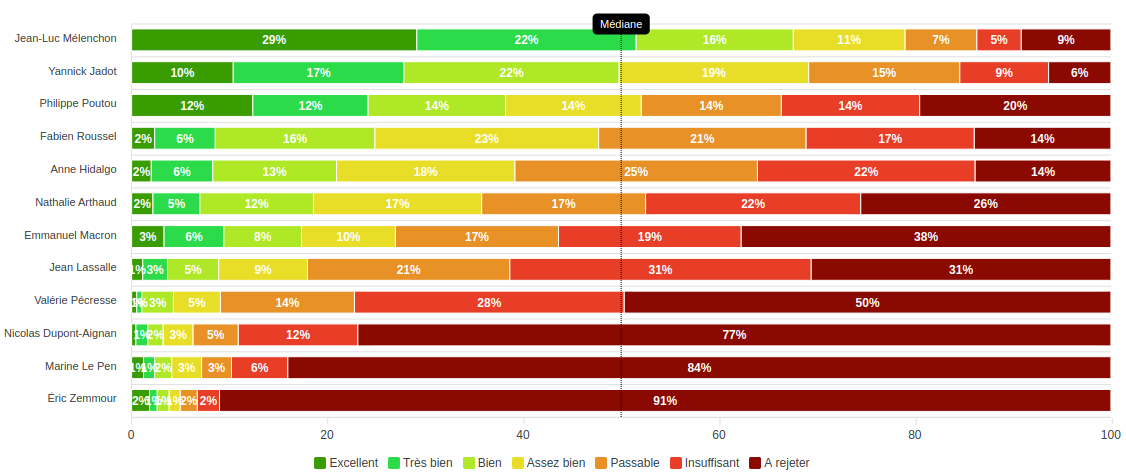
\includegraphics[scale=0.35]{data/profileUAV}
	\end{figure}
	
	The grade vector associated to the candidate Jean-Luc Mélenchon is composed for: $29\%$ of Excellent grades, $22\%$ of Very good, $16\%$ of Good, $11\%$ of Average, $7\%$ of Mediocre, $5\%$ of Inadequate and for $9\%$ of To be rejected.
	Because it is the winner of the complete profile this alternative will be our $j_0$ and its complete grade vector will be formed following the same proportions: $29\%$ of $\delta_7$, $22\%$ of $\delta_6$, $16\%$ of $\delta_5$, $11\%$ of $\delta_4$, $7\%$ of $\delta_3$, $5\%$ of $\delta_2$ and for $9\%$ of $\delta_1$.
	We follow the same reasoning for the other grade vectors in order to have the complete profile.
	
	Given $m=12$ alternatives we fix a value of $n$ and see what is the probability that $j_0$ is not in $K$ for $k$ from $1$ to $5$. Using the same reasoning as in the previous experiment we repeat this a total of $1,000,000$ times and we average over the probability. After that we increase $n$ and repeat the same experiment. We note that the probability decreases dramatically as $n$ increases so, although we varied $n$ from $10$ to $1500$, in \Cref{fig:MJelicitationUAV} we show the results only for a limited number of $n$ values.
	\Cref{tab:MJelicitationUAV} shows the data for the same values of $n$, the complete dataset can be found at \url{https://github.com/xoxor/elicitationMJ}. We see that when we have $n=50$ voters by asking $k=3$ questions per voter already we have an almost zero probability of not electing $j_0$. This result is obtained by asking $2$ questions per voter when $n=100$ and $1$ question when $n=500$.
	
	We conclude that in small profiles with few voters this method can pose a serious risk of not electing the "correct" alternative unless many questions are asked. This risk, however, is almost absent for elections in which a large number of voters are involved. \commentOC{You should be more careful about this conclusion, because it is unclear that these experiments really cover all the situations that could happen and that the probabilities of being wrong would always be so low. (I believe that the claim is correct but I wouldn’t say that these experiments show it conclusively by themselves, even though they are a step in that direction.)}
	
	\begin{figure}
		\centering
		\caption{Average probability of missing the winner using a real case distribution of preferences, given $m=12$ for $n\in \{10,25,50,100,250,500\}$ and $k\in \intvl{1,5}$.}
		\label{fig:MJelicitationUAV}
		\begin{tikzpicture}[scale=1.2]
			\pgfplotsset{
				every axis legend/.append style={
					at={(0.5,1.1)},
					anchor=south
				},
			}
			\begin{axis}[
				%	y=8,
				xlabel=$k$,
				ylabel=Avg. Prob. of Miss.,
				table/col sep=comma,
				legend columns=3,
				%	ytick={0,2,4,6,8,10},
				%	xtick distance=10,
				%	ytick distance=2,
				%	xtick pos=left,
				ymajorgrids=true,
				ytick style={draw=none},
				ymin=0,
				ymax=0.8,
				xmin=1,
				xmax=5,
				yticklabels={0,2,4,6,8,10},
					legend style={font=\scriptsize}
				]
				
				\addlegendimage{mark=halfsquare right*,brown,mark size=2}
				\addlegendimage{mark=diamond*,red,mark size=2}
				\addlegendimage{mark=pentagon*,cyan,mark size=2}
				\addlegendimage{mark=halfcircle*,violet,mark size=2}
				\addlegendimage{mark=*,pink,mark size=2}
				\addlegendimage{mark=triangle*,green,mark size=2}
				\addlegendimage{mark=halfsquare left*,blue,mark size=2}
				\addlegendimage{mark=square*,teal,mark size=2}
				\addlegendimage{mark=halfsquare*,magenta,mark size=2}
				
				
				\addplot[thick, mark=halfsquare right*, mark size = {2}, mark indices = {3}, brown] table [x=k, y=p10]{data/electiontableFig.dat};
				\addlegendentry{n=10}
				\addplot[thick, mark=diamond*, mark size = {2}, mark indices = {3}, red] table [x=k, y=p25]{data/electiontableFig.dat};
				\addlegendentry{n=25}
				\addplot[thick, mark=pentagon*, mark size = {2}, mark indices = {2}, cyan] table [x=k, y=p50]{data/electiontableFig.dat};
				\addlegendentry{n=50}
				\addplot[thick, mark=halfcircle*, mark size = {2}, mark indices = {2}, violet] table [x=k, y=p100]{data/electiontableFig.dat};
				\addlegendentry{n=100}
				\addplot[thick, mark=*, mark size = {2}, mark indices = {1}, pink] table [x=k, y=p250]{data/electiontableFig.dat};
				\addlegendentry{n=250}
				\addplot[thick, mark=triangle*, mark size = {2}, mark indices = {1}, green] table [x=k, y=p500]{data/electiontableFig.dat};
				\addlegendentry{n=500}
%				\addplot[thick, mark=halfsquare left*, mark size = {2}, mark indices = {1}, blue] table [x=k, y=p1000]{data/electiontableFig.dat};
%				\addlegendentry{n=1000}
%				\addplot[thick, mark=square*, mark size = {2}, mark indices = {1}, teal] table [x=k, y=p1500]{data/electiontableFig.dat};
%				\addlegendentry{n=1500}
				
			\end{axis}
		\end{tikzpicture}
	\end{figure}
	
	
	\begin{table}
		\centering
		\captionsetup{type=table}
		\caption{Average probability of missing the winner using a real case distribution of preferences, given $m=12$ for different values of $k$ and $n$.}
		\label{tab:MJelicitationUAV}
		\begin{tabular}{S[table-figures-integer=1, table-figures-decimal=0]S[table-figures-decimal=2]S[table-figures-decimal=2]S[table-figures-decimal=2]S[table-figures-decimal=2]S[table-figures-decimal=2]S[table-figures-decimal=2]}
			\toprule
			{$k$} & {avg $\mathcal{P}_{n=10}$} & {avg $\mathcal{P}_{n=25}$}& {avg $\mathcal{P}_{n=50}$}& {avg $\mathcal{P}_{n=100}$}& {avg $\mathcal{P}_{n=250}$} & {avg $\mathcal{P}_{n=500}$} \\
			\midrule		
			1	&	0.705851	&	0.495156	&	0.336408	&	0.167265	&	0.033418	&	0.004053	\\
			2	&	0.503269	&	0.218081	&	0.066655	&	0.008869	&	0.000117	&	0.00	\\
			3	&	0.339681	&	0.095145	&	0.008971	&	0.000149	&	0.00	&	0.00	\\
			4	&	0.184584	&	0.035866	&	0.000723	&	0.000001	&	0.00	&	0.00	\\
			5	&	0.069446	&	0.0099	&	0.000025	&	0.00	&	0.00	&	0.00	\\				
			\bottomrule
		\end{tabular}
	\end{table}
	
	\section{Conclusions}
		In this paper we analyzed a procedure proposed by the association \textit{Mieux Voter} and used in a real life application by \textit{LaPrimaire.org} for eliciting judgments of a set of voters over a set of alternatives.
		The procedure consists of randomly asking each voter to judge $k$ candidates on the $m$ available. The $k$ alternatives with the best medians are then presented to all voters in a second round of voting, and the best alternative is selected by \ac{MJ} as the winner.
		We have proven that given a complete profile it is possible to find an incomplete profile (such that a possible completion is equal to the considered profile) with a different winner from the complete profile.
		We also showed that the probability of this happening depends on the profile considered. 
		
		Moreover, we have performed experiments on profiles in which each grade vector has a randomly generated distribution of grade. Fixing the number of voters, we analyzed how much of the grade vector we must know in order for the probability missing the winner to be low.
		We have also considered a profile created from the grade distribution of a real voting scenario. We have found that the probability of not selecting the winner of the complete profile greatly decreases as the number of voters increases, making this method suitable for elections with large numbers of voters but less appropriate for small profiles.
		
		Future work on this topic could investigate the manipulability of this elicitation process. Especially on the side of the "analyst" who is in charge of questioning voters and how she can potentially manipulate the outcome by asking particular questions to specific groups of voters. For example, if she knows that voters in a given electoral district tend to vote predominantly for a given party she may decide never to ask those voters about that party's candidate (or vice-versa depending on the party she favors). 
		
		Another step might involve the explainability of this process to voters. In fact, voters may not understand how judging only one person gives a good approximation of the result that would be obtained by asking for the full profile. Also, they may not appreciate judging a random candidate and not their favorite.
		
		The code to reproduce the experiments in this article and the files with the reported data are available at \url{https://github.com/xoxor/elicitationMJ}.
	